\chapter{Results}
We test each of the specified variables over a range of values to examine trends in the reconstruction speed and overall accuracy. Unless otherwise noted, the default values for each simulation are listed in Table \ref{tab:def_vals}. Our error bars represent one standard deviation away from the mean and are calculated under the assumption of Gaussian noise. We assume this to be a good approximation of the true noise distribution based on the central limit theorem of statistics ***(make sure you've explained).\\

\begin{table}[h]
    \centering
    \begin{tabular}{|c|c|c|c|c|c|c|c|}
    \hline
    Variable: & Precision & Total hits & Hits used & P-value & $\eta'$-tolerance & $\sigma_{sp}$ & $a$ \\
    \hline
    Value: & single & 5 & 5 & 0.01 & 1.0 & 1 mm & 0.22 \\
    \hline
    \end{tabular}
    \caption{Default values used in computation}
    \label{tab:def_vals}
\end{table}

\section{Power}
To measure the power our hardware uses when running, we use the WITRN U2 USP Power Monitor\cite{WITRN}. Our original estimate for how much power usage would be acceptable aboard a telescope array was about 50 W based on past experience. We tested the Raspberry Pi's power usage and found that it ranged from about 2.52 W when idle to 2.74 W on average after running the program for a few hours. The differential power usage, found by subtracting the idle power from the power running the reconstruction algorithm, was 0.23 W on average. Though our USB monitor did not allow us to calculate its standard deviation, our maximum total and differential powers were 4.82 W and 2.30 W, respectively, which are both an order of magnitude less than our estimated power budget. We expect that the hardware in the telescope design will be similar to the raspberry pi, so it is likely that the true power used will be similar to these values.

\section{Precision}
The precision of our floating point values refers to how many bits we use in calculation. We use single-precision (32-bit) \texttt{float} values and double-precision (64-bit) \texttt{double} values in our calculations, and test them against each other. The results of our test runs are shown in Table \ref{tab:floatvdouble}. We see that we get slightly less accuracy on average when using float values rather than double values, but there is a large overlap in the two margins of error, so this is not a very statistically significant result. However, we also see a large decrease in reconstruction speed when using double values compared to floats. This is an expected result, as basic operations take longer for 64-bit values than for 32-bit values regardless of the hardware. This effect is less pronounced on Cassini as it has an out-of-order processor which can use its idle clock cycles to perform instructions for future use, decreasing the overall runtime. Unfortunately, the raspberry pi is an in-order processor and does not have such capabilities, so it is best that we use single-precision values in our final version of the program to increase the throughput.

\begin{table}[h]
    \centering
    \begin{tabular}{|c|c|c|}
        \hline
        Precision &  Single & Double \\
        \hline
        Accuracy (\%) & 86.12 $\pm$ .12 & 86.15 $\pm$ .10 \\
        \hline
        Throughput ($\gamma/sec$) & \num{5.08 \pm 0.70 e5} & \num{3.85 \pm .51 e5} \\
        \hline
    \end{tabular}
    \caption{Speed and accuracy results for single and double precision values}
    \label{tab:floatvdouble}
\end{table}

\section{Parallelism}
We test our algorithms' parallelism on Cassini as it has more cores. This speedup is calculated for both latency and throughput. Latency is defined here as the inverse of the execution speed: $L = \frac{1}{v} = \frac{T}{W}$, where $v$ is the execution speed, $T$ is the program's runtime, and $W$ is the work done by the program. The speedup in latency between programs 1 and 2 is then defined by $S_L = \frac{L_1}{L_2} = \frac{T_1 W_2}{T_2 W_1}$. As the work done by our program is approximately the same each time, this simplifies to $S_L = \frac{T_1}{T_2}$. In this case, $T_1$ is our base runtime, with only one core, while $T_2$ ranges from one to 24, the max number of cores on Cassini. The results are shown in Figure \ref{fig:latency_speedup}.

We define throughput here as the execution rate of a task: $Q = \rho v A = \frac{\rho A}{L}$, where $\rho$ is the number of stages in the pipeline and $A$ is the number of processors available. The latency in throughput is then $S_Q = \frac{Q_2}{Q_1} = \frac{\rho_2 A_2}{\rho_1 A_1} S_L$. Since $\rho$ is the same for each run of the program, $S_Q = \frac{A_2}{A_1} S_L$, which is shown in Figure \ref{fig:through_speedup}. We can see that we have near-linear speedup when the number of cores is small, but still have an overall linear trend at higher numbers of cores. This indicates that our program scales well with increased execution capacity.

\begin{figure}
    \centering
    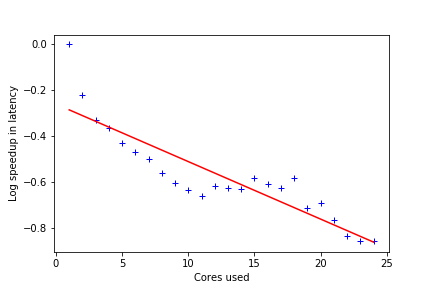
\includegraphics[width=0.7\textwidth]{graphs/Cassini_latency_speedup.png}
    \caption{Speedup of reconstruction algorithm in latency.}
    \label{fig:latency_speedup}
\end{figure}

\begin{figure}
    \centering
    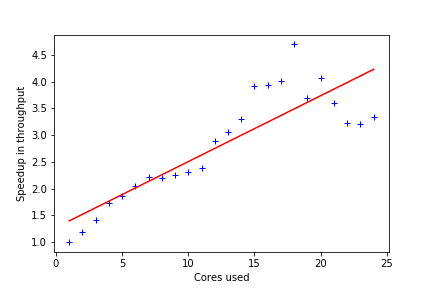
\includegraphics[width=0.7\textwidth]{graphs/Cassini_throughput_speedup.png}
    \caption{Speedup of reconstruction algorithm in throughput.}
    \label{fig:through_speedup}
\end{figure}

%%% Number of hits

\section{Total hits used}
\label{totalhits}
To ensure that our program is behaving correctly, we investigate its behavior using events with increasing numbers of hits. We can see from Figure \ref{fig:hits_speed} that our throughput decreases exponentially with increasing numbers of simulated hits. While not ideal, this is an improvement on our original estimate of a factorial increase in computation time for increasing hits. Though, theoretically, the worst-case time complexity of our program remains the same as in the iterative version, tree search improves the average-case complexity of our search algorithm and displays improved performance over a large number of simulated photons.

In plotting the accuracy of our program for increasing numbers of hits (Figure \ref{fig:hits_acc}) we find some interesting results in that the accuracy has a peak at 5 simulated hits. It is unclear from the algorithm exactly why this is, but it is possible that increasing the number of hits past a certain point introduces more error, while having fewer hits to work with does not constrain the problem enough. If a similar trend holds for testing on more accurate simulators, we may consider weighting our angle reconstructions based on these probabilities, using them as a prior when we calculate our final source position from the available angle reconstructions.

\begin{figure}
    \centering
    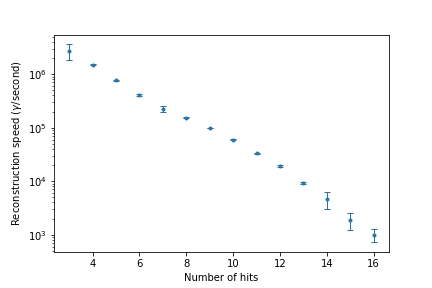
\includegraphics[width=0.7\textwidth]{graphs/pi_hits_speed.png}
    \caption{Reconstruction speed with increasing numbers of hits per event}
    \label{fig:hits_speed}
\end{figure}

\begin{figure}
    \centering
    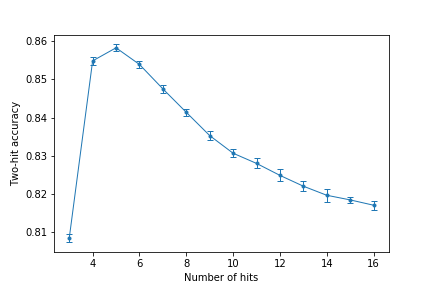
\includegraphics[width=0.7\textwidth]{graphs/pi_hits_acc.png}
    \caption{Reconstruction accuracy with increasing numbers of hits per event}
    \label{fig:hits_acc}
\end{figure}

%%% Hits v hits Used

\section{Reconstructed hits}
\label{reconhits}
We next investigate our program's performance varying both the total number of hits for each event and the number of hits we use in our reconstruction. When we stop computation at a certain number of hits, the ordering with the lowest $\chi^2$-value we have found so far becomes our chosen reconstruction. While this would in theory decrease the computation time for each event, it also has the potential to also decrease the overall accuracy due to the fact that we are not using all the information available to us in our reconstruction. To determine how big the trade-off is in accuracy and reconstruction speed, we simulate each possible combination of total hits versus reconstructed hits and plot one line for each type of event. So, each set of events with N hits is its own line, and each point in the line indicates a different number of hits used in its reconstruction. The results in speed and accuracy are displayed in Figures \ref{fig:hits_v_hitsUsed_speed} and \ref{fig:hits_v_hitsUsed_acc}, respectively.

As expected, our throughput decreases with increasing hits used in reconstruction while accuracy increases. For throughput, this trend is especially pronounced for events with more hits, and seems to drop sharply around 10-12 hits. The opposite is true of our accuracy, with gains tailing off at around 6-8 hits. Beyond this number, using more hits in reconstruction only gives us marginal gains in accuracy while significantly decreasing our speed. It would be reasonable, therefore, to set a maximum number of reconstructed hits for all events, increasing our reconstruction speed by sacrificing a small amount of accuracy. It is not immediately clear from our data what the optimal cutoff value should be, as we would need the correct energy distribution of our source to predict any losses in our overall accuracy. In a real-world test setting, events with high numbers of hits are much less probable than events with low numbers of hits, so our losses in overall accuracy would likely be less severe than those predicted for a certain event type.

Despite these considerations, we can perform some preliminary calculations assuming a flat source distribution (i.e. all event types are equally probable), shown in Figure \ref{fig:hits_v_hitsUsed_resids}. For each possible cutoff value in reconstructed hits, we calculate the residual accuracy, or the accuracy lost by ignoring higher orders of hits. This way, we can decide how much accuracy we are willing to trade for an increase in speed and set the maximum cutoff accordingly. Similar calculations can be done for residuals in speed.

- *** should be run again on the pi\\
- *** possibly include the residual speed as well

\begin{figure}
    \centering
    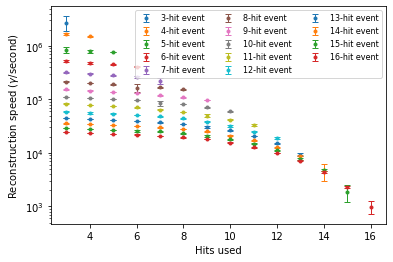
\includegraphics[width=0.7\textwidth]{graphs/pi_hits_v_hitsUsed_speed.png}
    \caption{Decrease in speed with hits used in reconstruction}
    \label{fig:hits_v_hitsUsed_speed}
\end{figure}

\begin{figure}
    \centering
    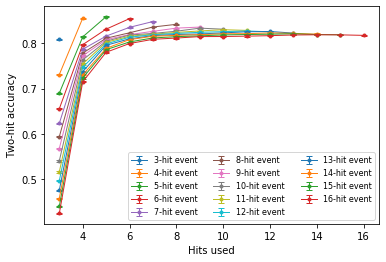
\includegraphics[width=0.7\textwidth]{graphs/pi_hits_v_hitsUsed_accuracy.png}
    \caption{Increase in accuracy with hits used in reconstruction}
    \label{fig:hits_v_hitsUsed_acc}
\end{figure}

\begin{figure}
    \centering
    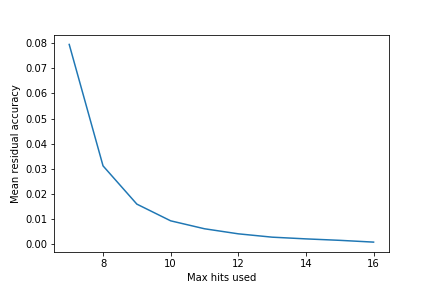
\includegraphics[width=0.7\textwidth]{graphs/mean_resid_acc.png}
    \caption{Residual accuracy for an increasing cutoff in reconstructed hits}
    \label{fig:hits_v_hitsUsed_resids}
\end{figure}

\section{Cutoff values}
\subsection{$\chi^2$ cutoff}
Changing the p-value of our calculation changes our certainty in our results. If we use a smaller p-value, we can be more certain that any orderings we exclude are truly bad ones, but we also cannot exclude as many orderings, so we expect that our speed will increase and our accuracy will decrease as our p-values get larger. Our results confirm this expectation, as shown in Figures \ref{fig:p_speed} and \ref{fig:p_acc}. Over our tested range of p-values, our accuracy has a range of about 5\%, while our reconstruction speed only changes by about 1-2\%. Based on these tests, it would be most efficient to choose one of the smaller p-values tested for our final calculations, as it would not significantly affect our overall runtime.

\begin{figure}
    \centering
    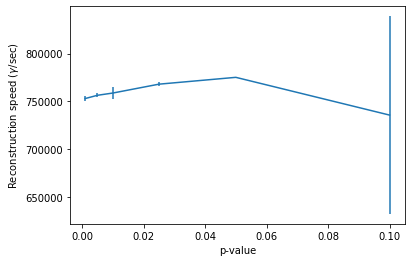
\includegraphics[width=0.7\textwidth]{graphs/pi_p_speed.png}
    \caption{p-value vs. reconstruction speed}
    \label{fig:p_speed}
\end{figure}

\begin{figure}
    \centering
    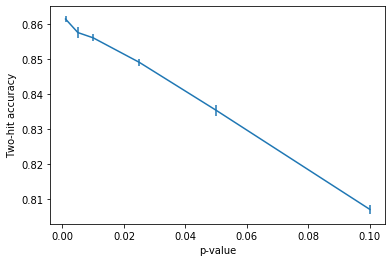
\includegraphics[width=0.7\textwidth]{graphs/pi_p_acc.png}
    \caption{p-value vs. reconstruction accuracy}
    \label{fig:p_acc}
\end{figure}

\subsection{$\eta'$ cutoff}
There is no clear trend in our results for $\eta'$ tolerance, shown in Figures \ref{fig:eta_speed} and \ref{fig:eta_acc}. Though there are sharp drops in reconstruction speed for certain $\eta'$ values, this could just as easily be due to processor error as a real trend in the data, and the large uncertainties would cast doubt on any trends perceived. In accuracy, there is similarly no clear trend, and the range is so small as to be insignificant for our purposes.

\begin{figure}
    \centering
    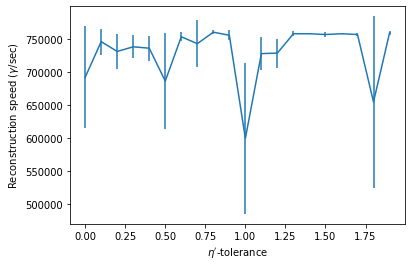
\includegraphics[width=0.7\textwidth]{graphs/pi_eta_speed.png}
    \caption{$\eta'$ tolerance vs. reconstruction speed}
    \label{fig:eta_speed}
\end{figure}

\begin{figure}
    \centering
    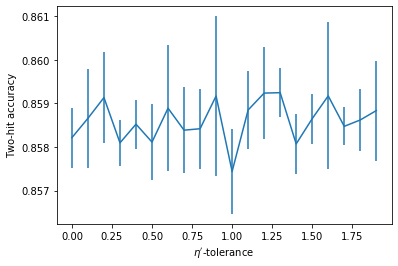
\includegraphics[width=0.7\textwidth]{graphs/pi_eta_acc.png}
    \caption{$\eta'$ tolerance vs. accuracy}
    \label{fig:eta_acc}
\end{figure}

\section{Noise}
We must input a noise level in our reconstruction calculations in order to get accurate results, but it is impossible to know the true noise level that we will see when the APT is operational. Thus, we test different levels of simulated noise and predicted noise to determine if there is any correlation between them.

\subsection{Predicted Noise}
We simulate different levels of predicted noise by changing the $a$ parameter in our energy calculations and the $\sigma_{sp}$ parameter in our spatial calculations, and our results are shown in Figures \ref{fig:predicted_speed} and \ref{fig:predicted_acc}. There are no significant trends in reconstruction speed when the simulated noise is changed, which stands to reason as our calculation is the same either way. The same goes for the accuracy of our predicted spatial noise, which has too small a range to be considered an effective parameter. However, the accuracy of our predicted energy noise does show a clear trend which flattens out as the predicted energy noise approaches the true energy noise. If we overestimate the noise, we see the same or very similar accuracy to a correct noise estimate, but if we underestimate the noise we see a severe decrease in accuracy. If this trend holds for more robust simulator data, it could be a good way to probe the true background noise when the telescope is in operation.

\begin{figure}
        \centering
        \begin{minipage}{0.49\textwidth} \centering
        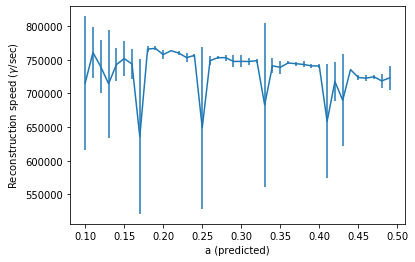
\includegraphics[width=\textwidth]{graphs/pi_enFactor_speed.png}
        \end{minipage}
        \begin{minipage}{0.49\textwidth} \centering
        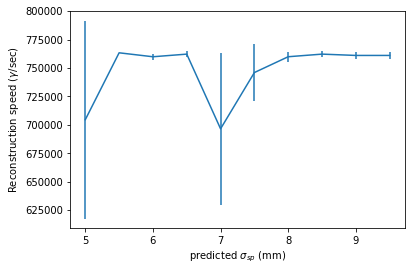
\includegraphics[width=\textwidth]{graphs/pi_spFactor_speed.png}
        \end{minipage}
        \caption{Reconstruction speed with increasing levels of predicted noise}
        \label{fig:predicted_speed}
\end{figure}

\begin{figure}
        \centering
        \begin{minipage}{0.49\textwidth} \centering
        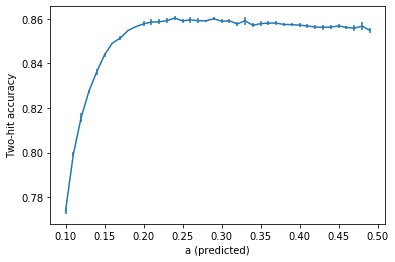
\includegraphics[width=\textwidth]{graphs/pi_enFactor_acc.png}
        \end{minipage}
        \begin{minipage}{0.49\textwidth} \centering
        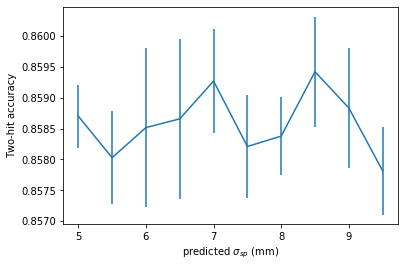
\includegraphics[width=\textwidth]{graphs/pi_spFactor_acc.png}
        \end{minipage}
        \caption{Reconstruction accuracy with increasing levels of predicted noise}
        \label{fig:predicted_acc}
\end{figure}

\subsection{Simulated Noise}
We also test our program's speed and accuracy with differing levels of simulated noise, shown in Figures \ref{fig:sim_speed} and \ref{fig:sim_acc}. We see fairly expected results, that there are no clear trends in reconstruction speed but that the accuracy goes down with increasing noise in our detected events. This is useful as a check on our toy model simulator, as less clear trends in the accuracy might prompt us to evaluate whether our simulator works as we expect it to.

\begin{figure}
        \centering
        \begin{minipage}{0.49\textwidth} \centering
        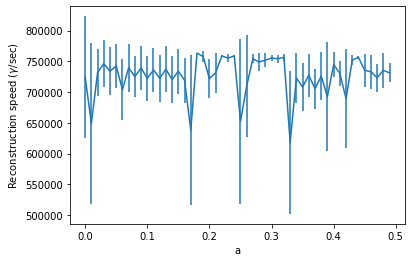
\includegraphics[width=\textwidth]{graphs/pi_enNoise_speed.png}
        \end{minipage}
        \begin{minipage}{0.49\textwidth} \centering
        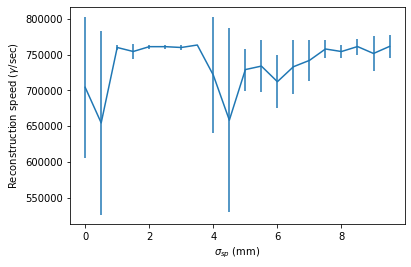
\includegraphics[width=\textwidth]{graphs/pi_spNoise_speed.png}
        \end{minipage}
        \caption{Reconstruction speed with increasing simulated noise level}
        \label{fig:sim_speed}
\end{figure}

\begin{figure}
    \centering
    \begin{minipage}{0.49\textwidth} \centering
        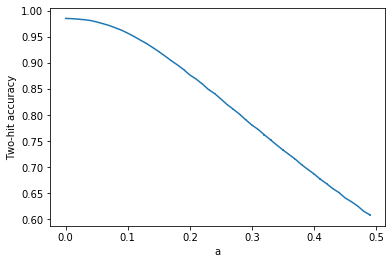
\includegraphics[width=\textwidth]{graphs/pi_enNoise_acc.png}
        \end{minipage}
        \begin{minipage}{0.49\textwidth} \centering
        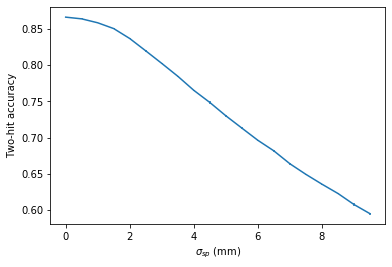
\includegraphics[width=\textwidth]{graphs/pi_spNoise_acc.png}
        \end{minipage}
        \caption{Reconstruction accuracy with increasing simulated noise level}
        \label{fig:sim_acc}
\end{figure}